\documentclass[12pt, a4paper]{article}
\usepackage{geometry}
\usepackage{tikz}
\usepackage[style=verbose]{biblatex}

\renewcommand\familydefault{\sfdefault}

\definecolor{spotifygreen}{HTML}{1DB954}

\usetikzlibrary{calc}
\usetikzlibrary{arrows.meta}
\usetikzlibrary{decorations.pathreplacing}
\usetikzlibrary{shapes}
\usetikzlibrary{positioning}

\tikzstyle{box}=[fill=black, solid, line width=0mm, text=white, rounded corners=2mm, font={\bfseries}, inner sep=3mm]    
\tikzstyle{sizedbox}=[box, text width=3cm, anchor=north, align=center]
\tikzstyle{link}=[->, >=latex, line width=.5mm, rounded corners, shorten >=1pt]
\tikzstyle{smalllink}=[->, >=latex, line width=.2mm, rounded corners, shorten >=1pt, dashed, gray]

\begin{filecontents}{references.bib}
@online{
    flux,
    title={In-Depth Overview: Flux},
    url={https://facebook.github.io/flux/docs/in-depth-overview},
},
@online{
    mpsc,
    title={Module futures::channel::mpsc},
    url={https://docs.rs/futures/latest/futures/channel/mpsc/index.html},
}
\end{filecontents}
\addbibresource{references.bib}

\begin{document}

\section{Data flow}

\subsection{Actions and events}

The application state can only be modified by dispatching \emph{actions}. Updates to the state produce \emph{events}, which \emph{listeners} can use to update the UI.

\begin{figure}[!h]

    \centering
    
    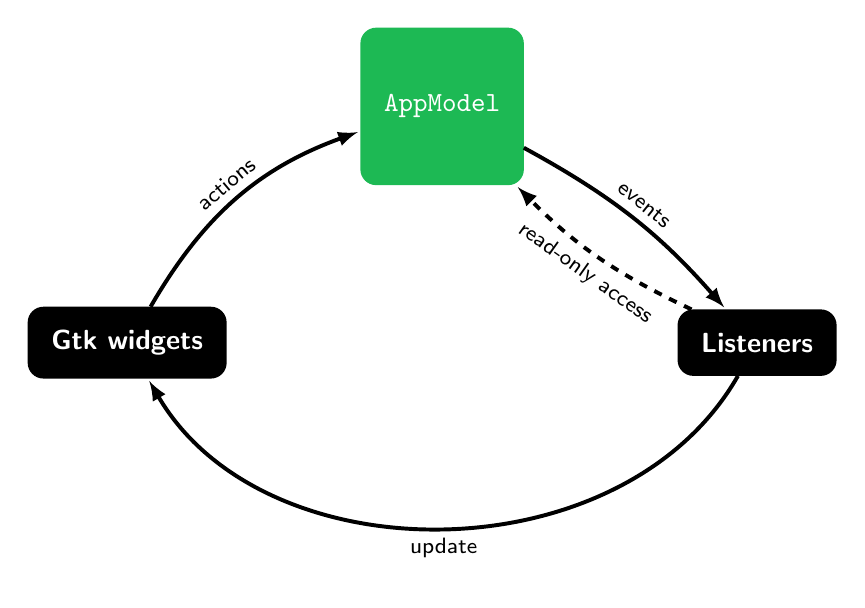
\begin{tikzpicture}

    \node[box, fill=spotifygreen, minimum height=2cm] (model) at (0, 0) {\ttfamily AppModel};
    \node[box] (ui) at (-4, -3) {Gtk widgets};
    \node[box] (listeners) at (4, -3) {Listeners};

    \draw[link] (ui) edge[bend left=20] node[above, sloped] {\footnotesize actions} (model);
    \draw[link] (model) edge[bend left=10] node[above, sloped] {\footnotesize events} (listeners);
    \draw[link] (listeners) edge[bend left=60] node[below, sloped] {\footnotesize update} (ui);
    \draw[link, dashed] (listeners) edge[bend left=10] node[below, sloped] {\footnotesize read-only access} (model);

    \end{tikzpicture}

    \caption{The data flow and and its relation to the UI}
    \label{fig:flow}

\end{figure}

Events can often help to have an idea of the current state. However, the \texttt{AppState} should be the only source of truth for the current state of the application. The \texttt{AppModel} enforces read-only access to that state.

This draws heavy inspiration from the Flux architecture\footcite{flux}; the one big difference here is that there is no way to automatically find out which portion of the UI should be updated. Instead, listeners are responsible for figuring out the updates to apply based on the events.

It should be noted that the app state is only readable from the main thread for simplicity. 

\subsection{A listener: the player subsystem}

Any element that wishes to update the state or react to changes from the state has to follow that same pattern. For instance, the ``player'' part of Spot receives \texttt{Commands} (mapped from events by a \texttt{PlayerNotifier}) to start playing music, and dispatches actions back the app through a \texttt{SpotifyPlayerDelegate} (see figure \ref{fig:player}). 

These two extra elements add some indirection so that the player is not too strongly coupled to the rest of the app (it does not and should not care about most events, afterall!). Moreover, those commands are handled in a separate thread where the player lives.

\subsection{Everything is just actions and events!}

In fact, widgets and their associated listeners (called \emph{components} throughout the codebase) form another similar subsystem that only communicate with actions and events.

\begin{figure}[!ht]
    \centering
    
    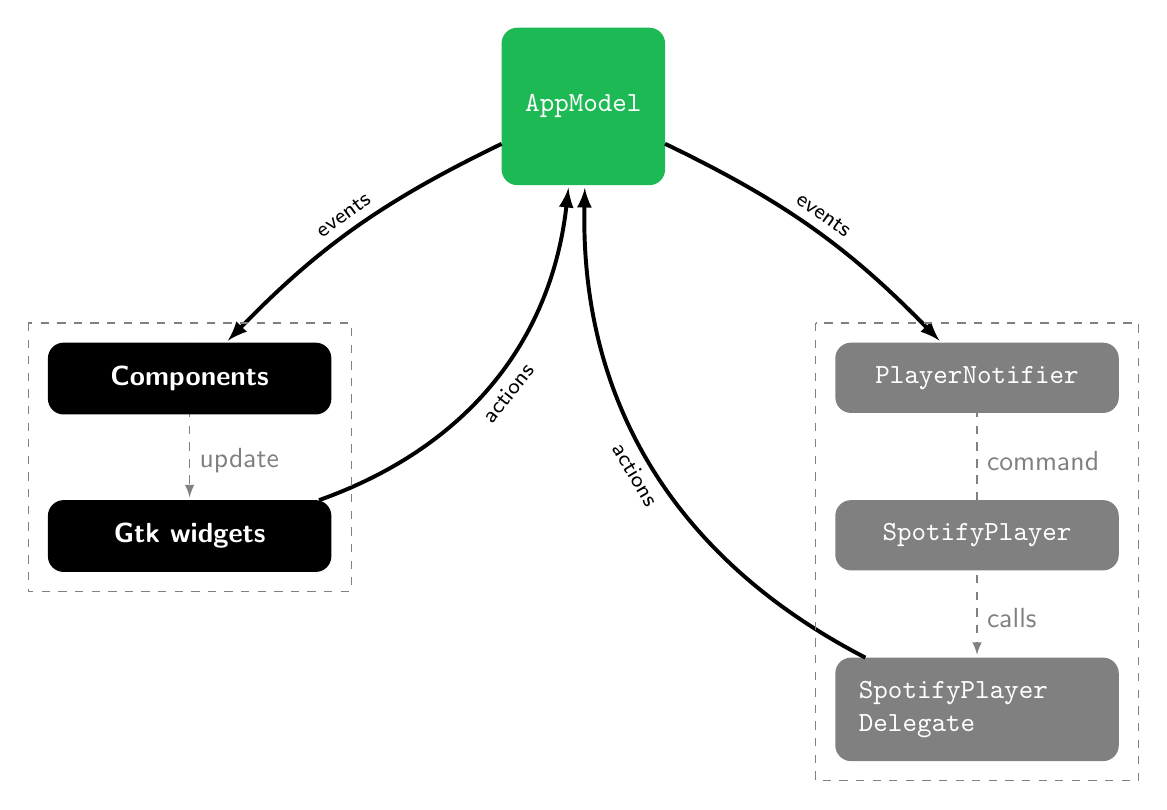
\begin{tikzpicture}

    \node[box, fill=spotifygreen, minimum height=2cm] (model) at (0, 0) {\ttfamily AppModel};

    \draw[smalllink] (-5, -3) node[sizedbox] (listeners) {Components}  
        -- +(0, -1.5) node[right] {update}
        -- +(0, -2) node[sizedbox] (ui) {Gtk widgets};

    \draw[smalllink] (5, -3) node[sizedbox, fill=gray] (notifier) {\ttfamily PlayerNotifier}
        -- +(0, -1.5) node[right] {command}
        -- +(0, -2) node[sizedbox, fill=gray] (player) {\ttfamily SpotifyPlayer}
        -- +(0, -3.5) node[right] {calls}
        -- +(0, -4) node[sizedbox, fill=gray] (delegate) {\parbox{\textwidth}{\ttfamily SpotifyPlayer Delegate}};

    \draw[link] (ui) edge[bend right=32] node[below, sloped] {\footnotesize actions} (model);
    \draw[link] (model) edge[bend right=10] node[above, sloped] {\footnotesize events} (listeners);

    \draw[link] (model) edge[bend left=10] node[above, sloped] {\footnotesize events} (notifier);
    \draw[link] (delegate) edge[bend left=32] node[below, sloped] {\footnotesize actions} (model);

    \draw[dashed, gray] ($(notifier.north west) + (-0.25, 0.25)$) rectangle ($(delegate.south east) + (0.25, -0.25)$);

    \draw[dashed, gray] ($(listeners.north west) + (-0.25, 0.25)$) rectangle ($(ui.south east) + (0.25, -0.25)$);


    \end{tikzpicture}

    \caption{The player subsystem}
    \label{fig:player}

\end{figure}


\subsection{Another listener: the MPRIS subsystem}

Similarly, the MPRIS subsystem follows that same pattern. It spawns a small DBUS server that translates DBUS messages to actions, and an \texttt{AppPlaybackStateListener} listens to incoming events.

One major difference is that the MPRIS server has its own state here, since the app state cannot be accessed from outside the main thread. That state, however, is shared between the server thread (the MPRIS state read when a DBUS message asks for it) and the main thread (the MPRIS state is updated by the listener). 

This is an alternative approach to the one used for the player subsystem, where yet another MPSC channel was used to bridge the gap between two threads.

To make sure this local state stays in sync, DBUS messages should not alter the local state directly -- instead, we should wait for a roundtrip through the app and incoming events.

\section{How actions are handled}

All actions being dispatched, synchronous or not, are eventually sent through an MPSC channel\footcite{mpsc}. The consumer on the other end of the channel is a future that will be executed by GLib. This allows Gtk to process \emph{all actions} at its own pace, as part of its main loop.

This is the only time that the app state is borrowed mutably -- to apply actions.

Note: futures are used a lot in the code to perform asynchronous operations such as calls to the Spotify API. To ease the use of futures, the dispatcher allows working with asynchronous actions, that is, futures that output one or more actions. Again, these futures are eventually handled in the main Gtk loop.

\section{Conventions for components}

Components are listeners dedicated to binding Gtk widgets so that they produce the right actions, and updating them when specific events occur.

The usual pattern adopted in the codebase is to have a model struct that defines accessors to the state and action-producing methods.

Because the state can only be borrowed immutably using the 
\texttt{AppModel}, there are sadly some hoops and loops to go through to work with \texttt{RefCells} if one wishes to avoid cloning data from the state.

\end{document}